\documentclass[a4paper, 12pt]{article}
\usepackage[utf8]{inputenc}
\usepackage[T2A]{fontenc}
\usepackage[english, russian]{babel}
\usepackage{amsmath, amsfonts, amssymb, amsthm, mathtools, forest}
\usepackage{graphicx}
\usepackage{wrapfig}
\usepackage{multirow}
\usepackage{forest}
\usepackage{float}
\usepackage{hyperref}
\usepackage{xcolor}

\title{Low Image Distortion Constrained Power Saving for OLED  Displays}
\author{Пучков Кирилл, ФУПМ, 777}
\date{15 April 2019}

\begin{document}

\maketitle

	Большинство современных смартфонов оснащены $OLED$-дисплеями. Уменьшение энергопотребления телефона всегда являлось приоритетной задачей производителя. В этой статье предложен метод малого искажения изображения, способствующий уменьшению энергопотребления дисплеем. Данный метод, в свою очередь, основан на двух методах: гамма-коррекции и масштабировании насыщения.
	
	Вначале мы изучим вклад последних двух методов на энергопотребление дисплея. В результате увидим, что изменяя значение $\gamma$ и насыщенность $S$ можно добиться значительного снижения энергозатрат, получив на выходе измененную картинку, слабо отличимую от оригинала. Однако низкое $\gamma$-значение и высокая насыщенность могут исказить картинку до неузнаваемости, поэтому мы используем формулу цветового различия $CIEDE2000$ и средний индекс структурного сходства $MSSIM$(Mean Structural Similarity Index) для определения эффективности нашего подхода.
	
\newpage
\section*{Вступление}

	Мобильные устройства можно рассматривать, как множество разнообразных элементов: центральный процессор, дисплей, $Wi-Fi$-интерфейс-контроллер, $Bluetooth$ адаптер, $GPS$, аудио и прочие. Известно, что процессор, экран и беспроводной сетевой интерфейс  самые энергозатратные составляющие.
	
	Экраны обычно делят на 2 группы: эмиссионные и неэмиссионные. Эмиссионные дисплеи сами преобразуют электрическую энергию в свет, а неэмиссионные используют оптические эффекты для преображения света в графический рисунок.
    
    $OLED$ (Organic Light Emitting Diode) — органические светодиоды эмиссионного типа. Благодаря своей структуре каждым пикселем можно управлять отдельно. Каждый пиксель, в свою очередь, состоит из малейших суб-пикселей, которые могут излучать три базовых цвета: красный, зеленый, синий. Из опытов было получено, что пиксели разного цвета потребляют разное количество энергии.
    
\newpage
\section*{Предложенный метод}

\subsection*{Модель энергопотребления 
    OLED дисплеями}

	Для расчета энергопотребления содержимого OLED дисплея предложена формула энергопотребления содержимого дисплея на пиксельном уровне:
	
	\[P_{content}=\sum_{i=1}^n P_{pixel}^i= \sum_{i=1}^n (w_0+w_1\cdot R_i^{\gamma} + w_2\cdot G_i^{\gamma}+w_3\cdot B_i^{\gamma})\]
    
    Где:
    \begin{itemize}
    	\item $n$ - количество пикселей на экране
    	\item $w_0$ - потребление мощности каждого пикселя в выключенном состоянии ($\sum_i w_0$ — энергопотребление матрицы пикселей)
    	\item $R_{ith},G_{ith}, B_{ith} - 3$ составляющие цвета $i$-ого пикселя
    	\item $\gamma$ - гамма-значение содержимого дисплея в стандартной $RGB$-модели
    	\item $w_1:w_2:w_3 = 24:35:50$ - константы эффективности красного, зеленого, синего цветов соответственно (обратно пропорциональны эффективности мощности). В процессе старения экрана они меняются, но мы будем считать их константами 
    \end{itemize}
    
    Энергопотребление OLED дисплея определяется яркостью экрана и энергопотреблением его содержимого:
    
    \[P_{display}=L\cdot P_{content}+P_{base}\]
    
    Где:
    \begin{itemize}
    	\item $L$ - яркость экрана ($\in [0, 255]$)
    	\item $P_{base}$ - энергопотребление других элементов дисплея (например контроллера)
    \end{itemize}
    
\subsection*{Гамма-коррекция}

	Гамма-коррекция перераспределяет тональные уровни ближе к тому, как их воспринимают наши глаза. На 1 картинке верхняя строка показывает как воспринимается яркость человеческим глазом: при увеличении яркости в 2 раза (например, от $0.1$ до $0.2$) картинка действительно выглядит так, будто она в два раза ярче: изменения видны довольно отчетливо. Однако, когда мы говорим о физической яркости света, как, например, о количестве фотонов, выходящих из источника света, верную картину дает нижняя шкала. На ней удвоение значения дает правильную с физической точки зрения яркость, но поскольку наши глаза более восприимчивы к изменениям темных цветов, это кажется несколько странным.
	
	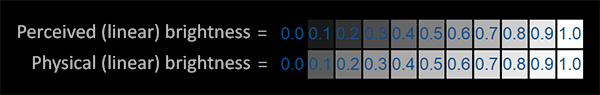
\includegraphics[scale=0.6]{1}
	
	Поэтому для записи изображения исходные значения пикселей преобразуются так, что в темной области диапазон цветов растягивается, а в светлой сжимается (гамма-кодирование).
	
	На картинке 2 красной сплошной линией показано изменения сигнала гаммой монитора. Идея гамма-коррекции заключается в том, чтобы применить инверсию гаммы монитора к окончательному цвету перед выводом на монитор. Снова посмотрим на график гамма-кривой, обратив внимание на еще одну линию, обозначенную штрихами, которая является обратной для гамма-кривой монитора. Мы умножаем выводимые значения цветов в линейном пространстве на эту обратную гамма-кривую (делаем их ярче), и как только они будут выведены на монитор, к ним применится гамма-кривая монитора, и результирующие цвета снова станут линейными. По сути мы делаем промежуточные цвета ярче, чтобы сбалансировать их затенение монитором.
	
	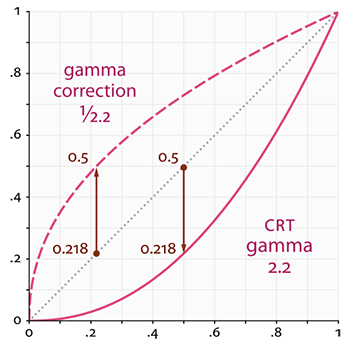
\includegraphics[scale=0.8]{2}

	Соотношение выходящего сигнала $L_{out}$ и входящего $L_{in}$  определяется формулой:
	
	\[L_{out} = L_{max}\cdot L_{in}^{\gamma}\]
	
	Где $L_{max}$ — максимальная яркость пикселей.
	
	Повышая значение $\gamma$, темные области изображения становятся более четкими. Понижая, наоборот, можно сделать светлые места более различными. На рисунке 3 применены 5 различных значений $\gamma$ к двум картинкам.
	
	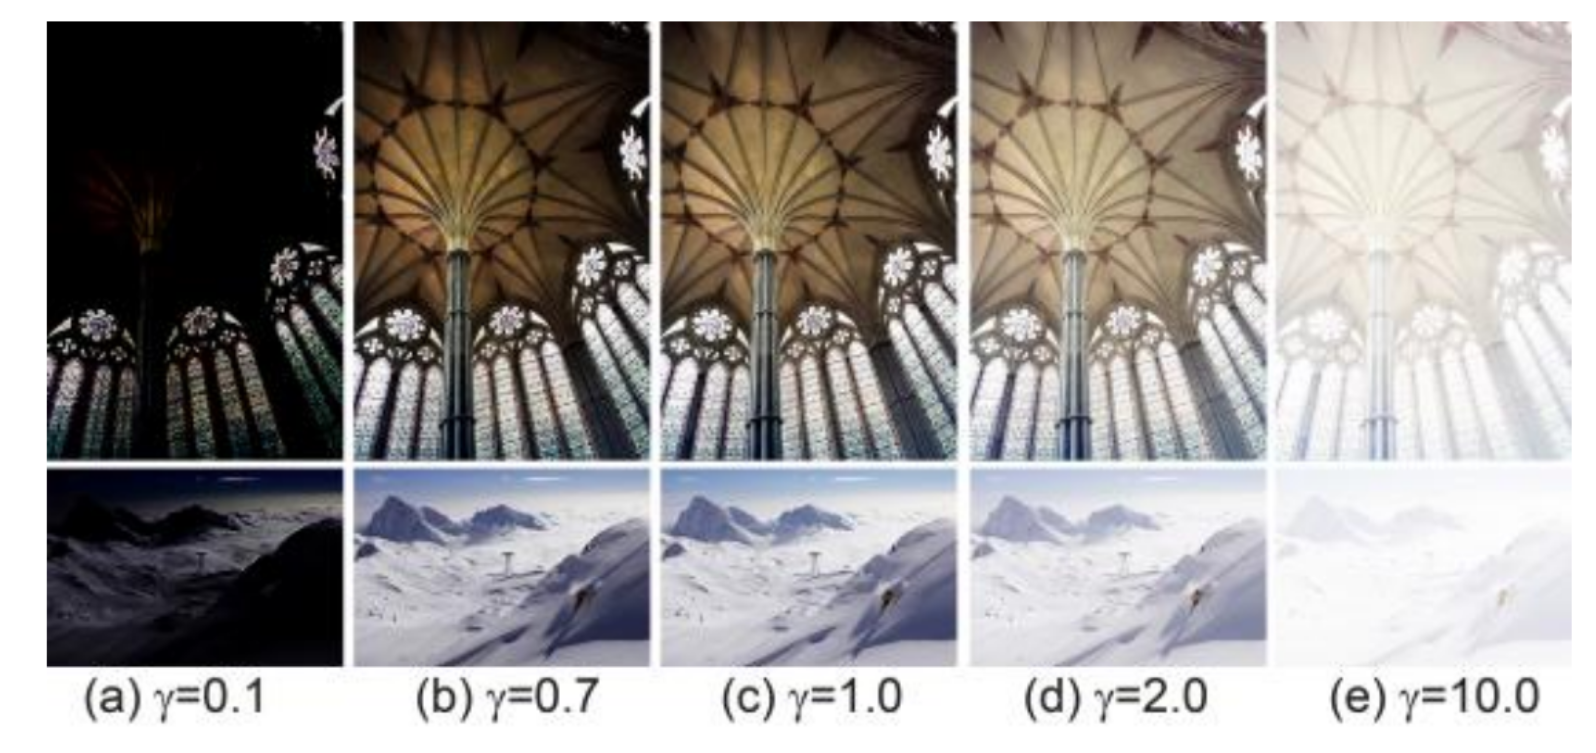
\includegraphics[scale=0.4]{3}
	
	Низкое значение $\gamma$ может значительно уменьшить энергопотребление. Однако темные регионы могут стать неразличимы и, следовательно, из-за сильного искажения картинка перестанет быть удовлетворительной. 
	
	Для сравнения двух рисунков применяются метод среднеквадратичного отклонения $MSE$ и вычисление пикового отношения сигнала к шуму $PSNR$. Однако данные алгоритмы не учитывают особенности человеческого восприятия. Для этого применяются другие методы измерения схожести: $CIEDE2000$ и $MSSIM$.
	
	Метод $CIEDE2000$:
	
	\[\vartriangle E=\sqrt{\left(\frac{\vartriangle L}{K_L\cdot S_L}\right)^2 + \left(\frac{\vartriangle C}{K_C\cdot S_C}\right)^2 + \left(\frac{\vartriangle H}{K_H\cdot S_H}\right)^2 + R_T}\]
	
	Где:
	\begin{itemize}
		\item $\vartriangle{E}$ - цветовая разница
		\item $\vartriangle L, \vartriangle C, \vartriangle H$ - арифметическая разница яркостей, насыщенности и тона соответственно
		\item $S_L, S_C, S_H$ - компенсация для  яркости, насыщенности и тона соответственно
		\item $K_L, K_C, K_H$ - параметрические константы
		\item $R_T$ - погрешность в синей области (очень мала)
	\end{itemize}
	
	Метод $MSSIM$ делит картинку на окна для того, чтобы учесть, что пиксели имеют сильную взаимосвязь, особенно когда они близки пространственно. Для вычисления $MSSIM$ изображение обводится окном фиксированного размера с центром по очереди в каждом пикселе (размер окна может быть разным). Математические ожидание, дисперсия и ковариация высчитываются для окон $x$ и $y$ одинакового размера. $\mu$ и $\sigma$ в формуле - это выборочное матожидание и выборочная дисперсия значений пикселей внутри окна.

	
	\[MSSIM(x, y)=\frac{1}{n}\sum_{i=1}^n \frac{(2\cdot \mu_{x}\cdot \mu_{y}+c_1)\cdot (2\cdot \sigma_{x y}+c_2)}{(\mu_{x}^2+\mu_{y}^2+c_1)\cdot (\sigma_{x}^2+\sigma_{y}^2+c_2)}\]
	
	Где:
	\begin{itemize}
	    \item $\mu$ — математическое ожидание
	    \item $\sigma^2$ - дисперсия
	    \item $\sigma$ - ковариация
	\end{itemize}
	
	$MSSIM \in [-1;1]$. Значение близкое к 1 значит, что обработанные изображения почти идентичны. И наоборот, значение близкое к -1 значит, что картинки сильно отличаются. На графике 2 показано отношение $MSSIM$ к $\gamma$.
	
	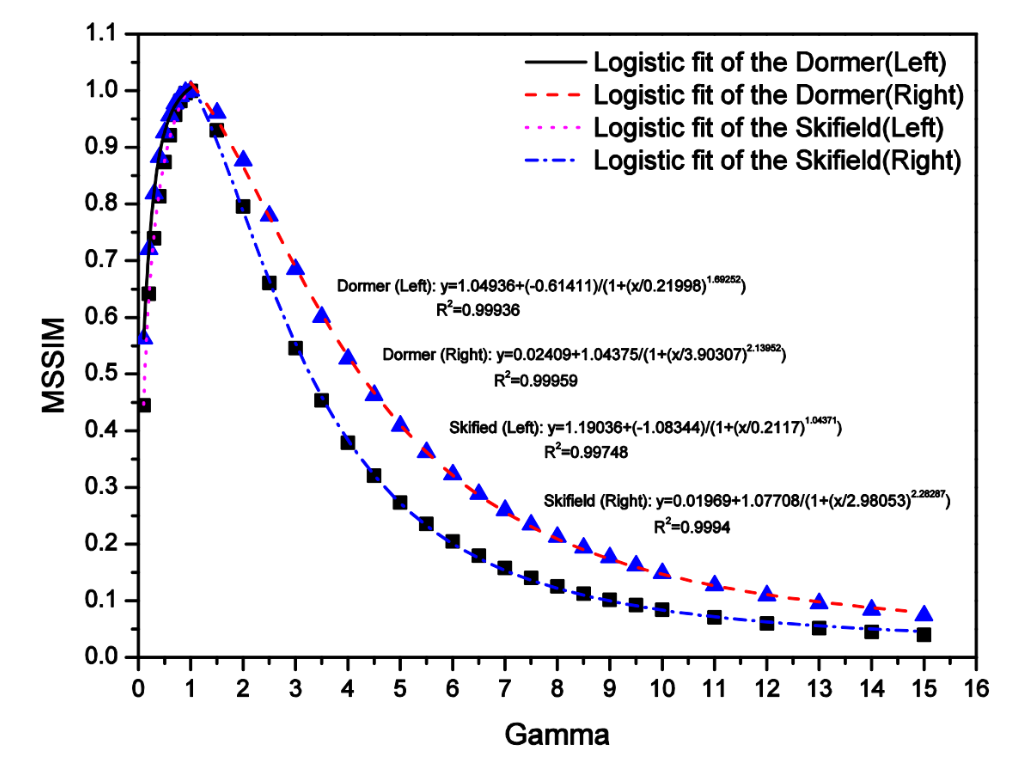
\includegraphics[scale=0.6]{4}
	
	Определим $M_0$ как порог восприятия $MSSIM$. Если значение $MSSIM$ больше либо равно $0,99$, то картинки нельзя различить. В нашем опыте примем $M_0 = 0.99$. 
	
	Для получения энергопотребления двух изображений, мы рассматривали гамма-коррекцию $\in [0.1;15]$, изменяя значение освещенности от 0 до 255. Повышенная освещенность изображения способствует улучшению четкости картинки, когда она затемнена. Однако высокая яркость требует больше энергии. С другой стороны, низкая освещенность может помешать конечному пользователю различать содержимое, особенно в затемненных областях.
	
	Поэтому предложена была идея затемнять картинку до наименьшего удовлетворительного порога, тем самым добившись уменьшения энергопотребления.
	
	Рассмотрим псевдокод метода гамма-корректировки $GC$.
	
	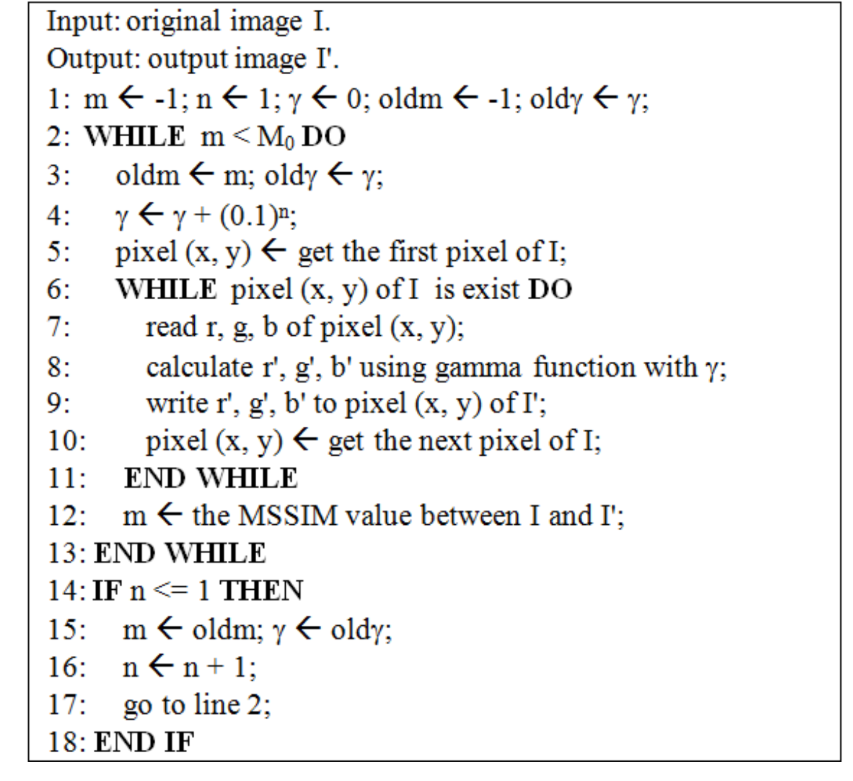
\includegraphics[scale=0.6]{5}
	
	Установим вначале значение $\gamma=0$, создадим выходное изображение. Увеличив $\gamma=\gamma+0.1$, изменим каждый пиксель картинки и перепишем в  выходное изображение. Будем увеличивать $\gamma$ до тех пора, пока $m < M_0$. Когда $m$ станет $\geq M_0$, вернемся на шаг назад и будем приближаться к нужному порогу сотыми: $\gamma+0.01$. Если в результате получено значение $\gamma < 1$, то мы получили похожее изображение с меньшим энергопотреблением. 
	
\subsection*{Масштабирование насыщенности}

    Насыщенность $S$ определим:
    
    \begin{equation*}
     S = 
     \begin{cases}
       0, \text{if} \max{(R, G, B)} = 0\\
       \dfrac{\max{(R, G, B)} - \min{(R, G, B)}}{\max{(R, G, B)}} &\text{, otherwise}
     \end{cases}
    \end{equation*}
    
    В цветовой модели $HSV$ насыщенность $S \in [0;1]$. Спектральный график насыщенности цвета от 0 до 1:
    
   
\includegraphics[scale=0.6]{6}
    
    Аналогично изменению гамма-коррекции, мы можем изменить в некоторых диапазонах насыщенность картинки, при этом оставив ее похожей на свой оригинал.
    
    Для измерения вклада насыщенности в энергопотребление картинки, мы меняли значение насыщенности, оставляя неизменными тон и яркость. Как показано на графике, энергопотребление изображений спадает с повышением насыщенности. Это становится еще более наглядно с повышением $\gamma$.
    
    Этот факт является одним из важнейших в данной статье. Руководствуясь логикой, менее насыщенный цвет становится ближе в белому, а энергопотребление у белого - максимально.
    
	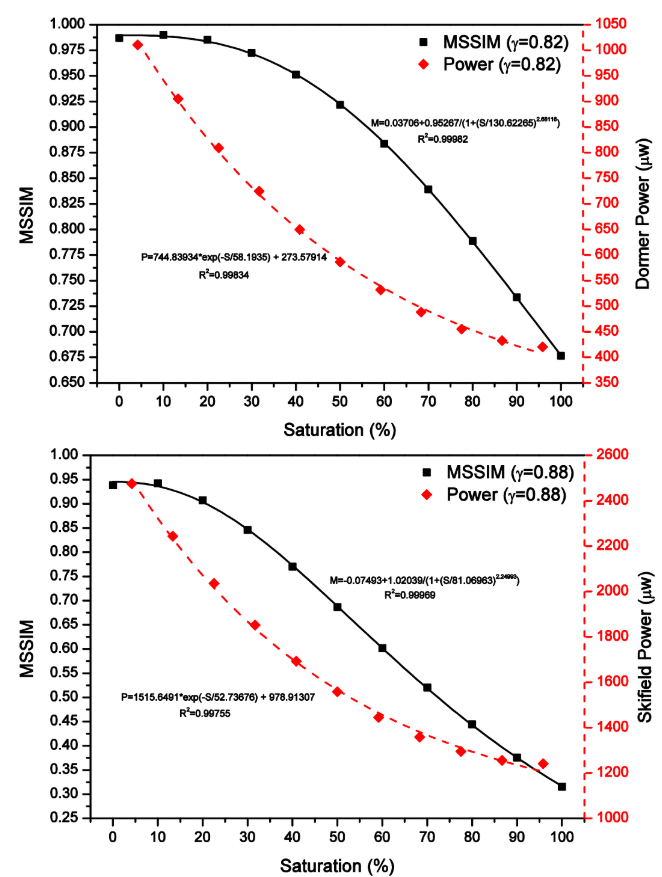
\includegraphics[scale=0.8]{7}
    
    Определим "порог насыщения" — максимальное значение насыщенности, при котором выходное изображение все еще приемлемо. Для этого рассмотрив псевдокод метода масштабирования насыщенности $SS$. 
    
    Установим значение $s' = 1$, то есть максимальное значение насыщенность (минимальное энергопотребление). Переведем каждый пиксель исходного изображения из $RGB$ модели в $HSV$. Увеличим исходное значение насыщенности пикселя, по полученному значению создадим новый пиксель и вернем в выходное изображение. После преображения всех пикселей сравним два изображения. Будем уменьшать $s'$, пока изображения не станут похожи. Аналогично методу гамма-коррекции, получим значение насыщенности с точностью до сотых. Если полученное значение насыщенности больше исходного, то мы получили более насыщенную картинку с меньшим энергопотреблением.
    
    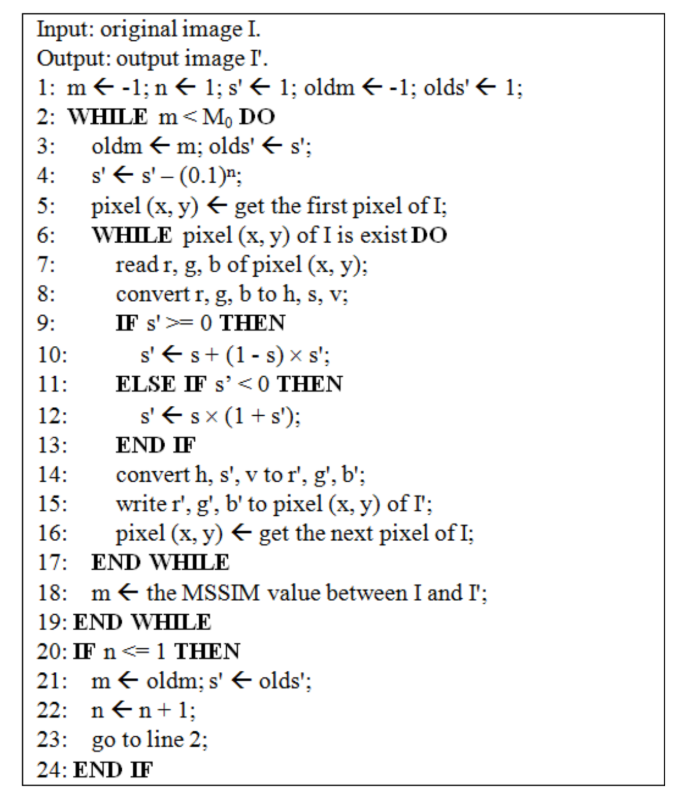
\includegraphics[scale=0.6]{8}
    
    
    Теперь применим последовательно оба метода(гамма-коррекции $GC$ и масштабирования насыщенности $SS$) в методе $GS$. Оба метода имеют временную сложность — $O(N)$ операций умножений и сложения, где $N$ — количество пикселей на экране телефона.
    Для ускорения программы можно искать значения $\gamma$ и $S_0$ путем двоичного поиска, а не итерационным. Также параллельное преобразование пикселей даст большой выигрыш во времени. 

\newpage
\section*{Результаты}

    Первый столбец - оригинальная картинка. Во втором столбце показаны допустимые искажения изображения методом гамма-коррекции. Как видно, картинки стали несколько темнее, по сравнению с изначальными.
    
    Третий столбец показывает картинки, после воздействия на них масштабирования насыщенности. Последний столбец показывает изображение, измененное методом $GS$. Оно более темно и насыщенно в сравнении с оригиналом. 
    
    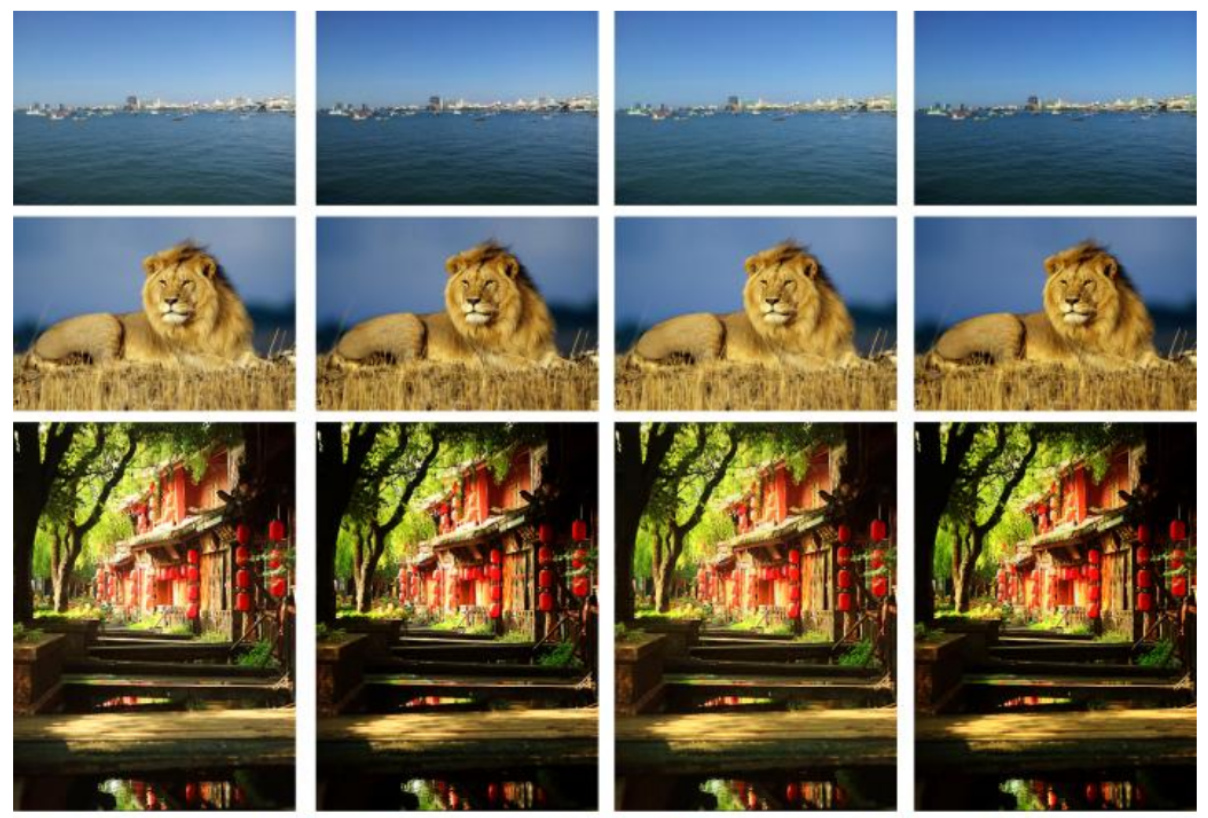
\includegraphics[scale=0.6]{9}
    
    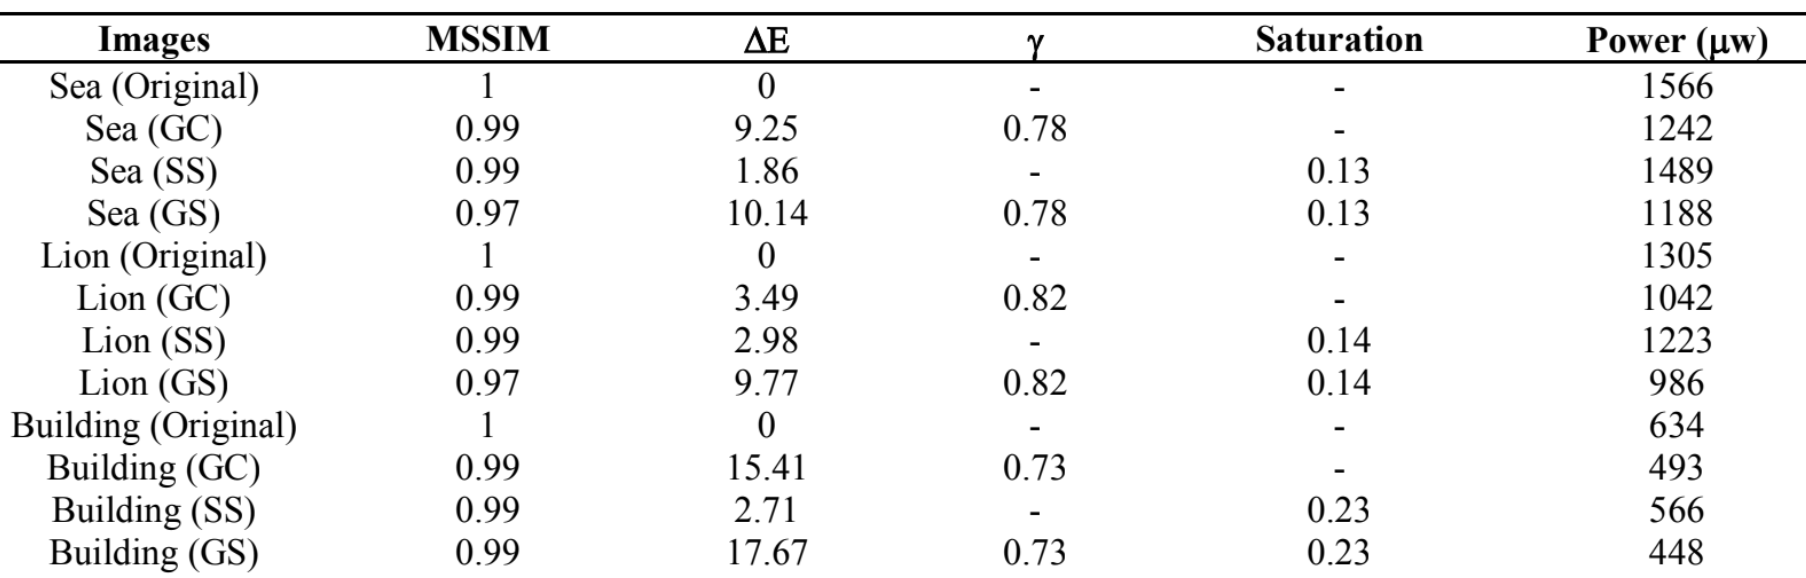
\includegraphics[scale=0.5]{10}
    
    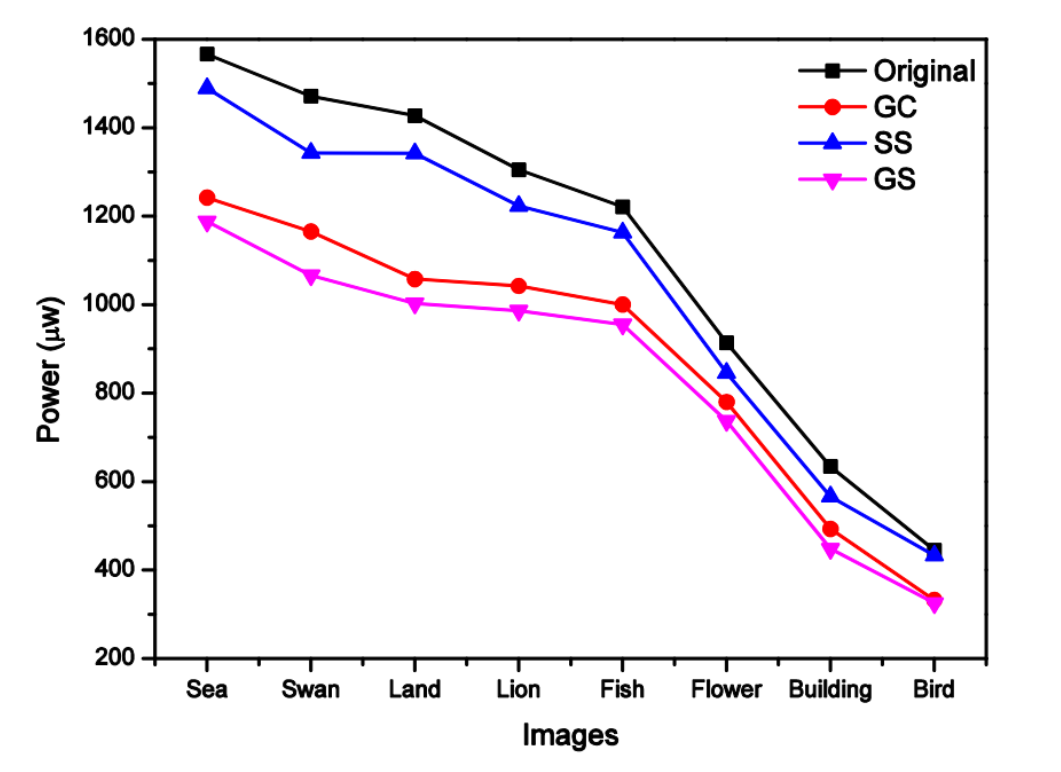
\includegraphics[scale=0.6]{11}

\newpage
\section*{Вывод}

	Метод гамма-коррекции и масштабирования насыщенности позволяет уменьшить энергопотребление $OLED$ дисплеями с малым искажением исходной картинки. Была предложена модель измерения мощности для эмиссионых экранов, а также 2 формулы проверки отличия полученного изображения от первоначального. Мы изучили вклад гамма-коррекции и масштабирования насыщенности в энергопотребление, а также продемонстрировали работу всех трех методов на изображениях. В результате наш метод дает значительный спад в энергопотреблении при позволительных потерях в качестве.
\end{document}
